\documentclass[a4paper,oneside, 11pt]{article}
\usepackage[margin=0.7in]{geometry}
\usepackage[cm-default]{fontspec}
\usepackage{xunicode}
\usepackage{xltxtra}
\usepackage{xgreek}
\usepackage{listings}
\usepackage{hyperref}
\usepackage{amsthm}
\usepackage{parallel,enumitem}
\lstset{basicstyle=\footnotesize\ttfamily,breaklines=true}
\setmainfont[Mapping=tex-text]{CMU Serif}
\usepackage{graphicx}
\usepackage{color}
\usepackage{mathtools, amsmath}
\usepackage{float}
\usepackage{caption}
\usepackage{titling}
\usepackage{tikz}
\definecolor{codegreen}{rgb}{0,0.6,0}
\definecolor{codegray}{rgb}{0.5,0.5,0.5}
\definecolor{codepurple}{rgb}{0.58,0,0.82}
\definecolor{backcolour}{rgb}{0.95,0.95,0.92}

\lstdefinestyle{mystyle}{
    backgroundcolor=\color{backcolour},   
    commentstyle=\color{codegreen},
    keywordstyle=\color{magenta},
    numberstyle=\tiny\color{codegray},
    stringstyle=\color{codepurple},
    basicstyle=\footnotesize,
    breakatwhitespace=false,         
    breaklines=true,                 
    captionpos=b,                    
    keepspaces=true,                 
    numbers=left,                    
    numbersep=5pt,                  
    showspaces=false,                
    showstringspaces=false,
    showtabs=false,                  
    tabsize=2
}
 
\lstset{style=mystyle}
\makeatletter
\def\maxwidth{%
  \ifdim\Gin@nat@width>\linewidth
    \linewidth
  \else
    \Gin@nat@width
  \fi
}
\makeatother

\makeatletter
\newcommand\xlongleftrightarrow[2][]{%
\ext@arrow 0059{\longleftrightarrowfill@}{#1}{#2}%
}
\def\longleftrightarrowfill@{%
\arrowfill@ ← \relbar → }
\makeatother




\pretitle{%
		\begin{center}
		\LARGE
		
\includegraphics[height=7cm]{pyrforos.png}\\[\bigskipamount]
}
\posttitle{\end{center}}
\title{\textbf{Αλγόριθμοι \\ 4η Σειρά Γραπτών Ασκήσεων}}
\author{ Ιωάννης Δάρας (\texttt{03115018, el15018@central.ntua.gr, daras.giannhs@gmail.com})
}
\date{“You probably know that arrogance, in computer science, is measured in nanodijkstras.” \\ —Alan Kay}

\newtheorem{lemma}{Λήμμα}
\begin{document}
\maketitle
\noindent\makebox[\linewidth]{\rule{\paperwidth}{0.4pt}}



\section{Άσκηση 1}

\subsection{Προεπεξεργασία}
Αρχικά, παρατηρούμε ότι ο γράφος των χρηστών μας δίνεται σε μορφή πίνακα γειτνίασης. Μια πιο βολική αναπαράσταση είναι η μετατροπή του σε λίστα γειτνίασης. Έτσι, θα μπορέσουμε να εκμεταλλευτούμε και στην εκτίμηση της πολυπλοκότητας ότι υπάρχουν m ακμές μεταξύ των χρηστών. Για να μετατρέψουμε τον πίνακα γειτνίασης σε λίστα γειτνίασης έχουμε πολυπλοκότητα $O(n^2)$. \bigbreak 

Στην ενότητα της διατύπωσης του αλγορίθμου θα δούμε ότι χρειαζόμαστε να τρέξουμε έναν αλγόριθμο εύρεσης ελάχιστων μονοπατιών. Παρατηρούμε όμως ότι το κόστος για δύο ακμές είναι το γινόμενο του κόστους των ακμών αντί για το άθροισμα τους και οι τιμές στις ακμές δεν είναι κόστη καθώς μικρή εμπιστοσύνη αντιστοιχεί σε μικρή τιμή. Με πιο αυστηρή μαθηματική ματιά, δεν βρισκόμαστε στον τροπικό ημιδακτύλιο ($\oplus \equiv min, \otimes \equiv +)$ για τον οποίο γνωρίζουμε αλγορίθμους εύρεσης συντομότερων μονοπατιών. Χρειάζόμαστε λοιπόν έναν μετασχηματισμό του γράφου ώστε να περάσουμε στον τροπικό ημιδακτύλιο. Ένας τέτοιος μετασχηματισμός είναι το $-log_{10}$ για τα βάρη. Με αυτόν τον μετασχηματισμό μεγάλες εμπιστοσύνες αντιστοιχούν σε μικρά ($0+\epsilon$ για κάποιο θετικό $\epsilon$) θετικά κόστη, μικρές εμπιστοσύνες αντιστοιχούν σε μεγάλα ($1 - \epsilon$ για κάποιο θετικό $\epsilon$) θετικά κόστη. Ακόμη, η σύνθεση ακμών για σχηματισμό μονοπατιών γίνεται από πολλαπλασιασμός πρόσθεση αφού:
$$
-\log_{10}(x_1 \cdot x_2) = (-\log_{10}x_1) + (-\log_{10}x_2) 
$$
Με βάση αυτές τις παρατηρήσεις, με τον μετασχηματισμό αυτό βρισκόμαστε στον τροπικό ημιδακτύλιο, για τον οποίο γνωρίζουμε αποδοτικούς αλγορίθμους εύρεσης ελάχιστων μονοπατιών.

\subsection{Διατύπωση αλγορίθμου}
Η βασική ιδέα είναι ότι για τον i χρήστη θα βρούμε τα συντομότερα μονοπάτια του προς κάθε χρήστη j χρησιμοποιώντας από 1 εώς k ακμές. Στη συνέχεια, για κάθε χρήστη j θα βρούμε το συντομότερο από αυτά τα μονοπάτια. Έστω ότι το μονοπάτι αυτό είναι το $p_t$, που ο συμβολισμός δηλώνει ότι το μονοπάτι αυτό χρησιμοποιεί ακριβώς t ακμές. Θα μετατρέψουμε το κόστος αυτού του μονοπατιού πίσω σε εμπιστοσύνη και θα δούμε αν είναι δεκτό μονοπάτι σύμφωνα με την μελέτη των ειδικών. Αν είναι, κάνουμε την αντίστοιχη πρόταση φιλίας. Αν δεν είναι, δοκιμάζουμε από τα συντομότερα μονοπάτια από τον i στον j που έχουμε υπολογίσει το συντομότερο που χρησιμοποιεί λιγότερες από l ακμές και συνεχίζουμε αναδρομικά μέχρι να μας τελειώσουν τα μονοπάτια ή μέχρι να γίνει η πρόταση φιλίας. \bigbreak 

Για την εύρεση των ελαχίστων μονοπατιών που χρησιμοποιούν όλων των ελαχίστων μονοπατιών που χρησιμοποιούν από 0 εώς k ακμές ένας τρόπος να δουλέψουμε είναι με δυναμικό προγραμματισμό. Συγκεκριμένα, σχηματίζουμε έναν πίνακα $DP[n][k]$ που στη θέση του $DP[u][j]$ θα πρέπει να έχει το κόστος του ελάχιστου μονοπατιού για να φτάσουμε από το i στο u χρησιμοποιώντας ως j ακμές. 
\bigbreak 
Η αναδρομική μας σχέση είναι:
$$
DP[v][j+1] = min \begin{cases}
DP[v][j] \\ min \big( \ DP[u][j] + w_{uv}  \  \forall u: (u, v) \in E \  \big) 
\end{cases}, \qquad \forall v \in V, \forall j \in \{0, ..., k-2\}
$$
Οι αρχικές συνθήκες είναι: $$DP[t][0] = \begin{cases}
0, \quad t = i \\
\infty, \quad t \neq i
\end{cases}$$

\bigbreak 

Στη συνέχεια, εφαρμόζουμε τη διαδικασία που περιγράψαμε. Για κάθε πιθανό φίλο, πρέπει να βρούμε, αν υπάρχει, αποδεκτό μονοπάτι. Ξεκινάμε από το $DP[u][k]$ που είναι το συντομότερο μονοπάτι που ξέρουμε. Βρίσκουμε το πλήθος των ακμών που αυτό χρησιμοποιεί κοιτώντας τον δείκτη j στον οποίο ισχύει 1η φορά ότι: $DP[u][k]\neq DP[u][j]$. Το πλήθος των ακμών που χρησιμοποιεί θα είναι $j+1$. Στη συνέχεια, το μετατρέπουμε σε εμπιστοσύνη με χρήση της σχέσης $$\textrm{trust} = 10^{-DP[u][j+1]}$$ και το συγκρίνουμε με το $\beta_{j+1}$. Αν δεν είναι αποδεκτό, συνεχίζουμε αναδρομικά μέχρι να βρούμε κάποιο αποδεκτό ή να μας τελειώσουν τα μονοπάτια.

\subsection{Ορθότητα αλγορίθμου}
Αρχικά, θα αποδείξουμε ότι το ελάχιστο μονοπάτι στον δεύτερο γράφο είναι αυτό που αντιστοιχεί στην μέγιστη εμπιστοσύνη στον πρώτο γράφο. Θα δουλέψουμε με άτοπο. Έστω ότι στον 1ο γράφο το ελάχιστο μονοπάτι αποτελείται από τις ακμές: $\{e_1, e_2, ..., e_t\}$. Αντί αυτού, διαλέγεται ένα μονοπάτι που αποτελείται από τις ακμές: $\{e_1, e_2, ..., e_t'\}$ (υποθέτουμε οτί διαφέρουν μόνο στην τελευταία ακμή χωρίς βλάβη της γενικότητας). Οι ακμές αυτές θα γίνουν στον 2ο γράφο: 
$$
\{-\log_{10}e_1, -\log_{10}e_2, ..., -\log_{10}{e_t} \}, \qquad \{-\log_{10}e_1, -\log_{10}e_2, ..., -\log_{10}{e_t'} \}
$$

Το μονοπάτια θα έχουν κόστη:
$$
w_1 = -\log_{10} \left(e_1 \cdot e_2 \cdot ... \cdot e_t\right), \qquad w_2 = -\log_{10} \left(e_1 \cdot e_2 \cdot ... \cdot e_t'\right),
$$
Για να επιλέχθηκε το 2ο αντί του 1ου σημαίνει ότι:
$$
w_2 > w_1 \iff 
$$
$$-\log_{10} \left(e_1 \cdot e_2 \cdot ... \cdot e_t'\right) > -\log_{10} \left(e_1 \cdot e_2 \cdot ... \cdot e_t\right) \iff
$$
$$
\log_{10}\left( \frac{1}{e_1 \cdot e_2 \cdot ... \cdot e_t'} \right) > \log_{10}\left( \frac{1}{e_1 \cdot e_2 \cdot ... \cdot e_t} \right) \iff 
$$
$$
e_1 \cdot e_2 \cdot ... \cdot e_t < e_1 \cdot e_2 \cdot ... \cdot e_t'
$$
το οποίο είναι άτοπο αφού αυτό εκφράζει την συνολική εμπιστοσύνη των μονοπατιών. \bigbreak 

Άρα, αποδείξαμε ότι δεδομένης της ορθότητας του αλγορίθμου υπολογισμού των συντομότερων μονοπατιών, ο αλγόριθμος μας υπολογίζει τα σωστά συντομότερα μονοπάτια στο νέο γράφο. \bigbreak 

Η ορθότητα του αλγορίθμου υπολογισμού των συντομότερων μονοπατιών προκύπτει άμεσα από την ορθότητα του αλγορίθμου Bellman ford, καθώς στην DP μορφή του, είναι ο αλγόριθμος Bellman ford για τις πρώτες k επαναλήψεις. \bigbreak 

%TODO ένα κομμάτι εδώ για το ότι ο Bellman ford είναι incremental.


Τέλος, πρέπει να αποδείξουμε την διάταξη που υποθέτει ο αλγόριθμος μας. Συγκεκριμένα, μετά τον υπολογισμό όλων των βέλτιστων μονοπατιών που χρησιμοποιούν ως t ακμές $\forall t \in \{2, ..., k\}$, εξετάζουμε τα μονοπάτια από τις περισσότερες ακμές προς τις λιγότερες. Αυτό σημαίνει ότι υποθέτουμε πως $$DP[i][t] \geq DP[i][t-1]$$. Αυτό προκύπτει άμεσα από τη σχέση: $$DP[v][j+1] = min(DP[v][j], ...), \qquad \forall v \in V$$ \bigbreak 
Από τα παραπάνω προκύπτει άμεσα η ορθότητα του αλγορίθμου που περιγράψαμε.
\subsection{Υπολογιστική πολυπλοκότητα}
Από την αναδρομικη σχέση που περιγράψαμε προκύπτει ότι χρειαζόμαστε $O(kn^2)$ για να υπολογίσουμε το DP αν χρησιμοποιούμε πίνακα γειτνίασης για την εύρεση των γειτόνων. Στη συνέχεια, πρέπει πιθανώς να ψάξουμε όλο τον πίνακα για να βρούμε πιθανούς φίλους και για κάθε στοιχείο του πίνακα πιθανώς χρειαζόμαστε backtracking στο DP μεχρι και k θέσεις. Έτσι, η πράξη αυτή έχει πολυπλοκότητα $O(k^2n)$. Έτσι, η συνολική υπολογιστική πολυπλοκότητα είναι:

$$
O(kn^2 + k^2n)
$$




\section{Άσκηση 2}
Ο αλγόριθμος του Dijkstra υπάρχει σε πολλές διαφορετικές παραλλαγές. Οι διαφοροποιήσεις υπάρχουν στο πως υλοποιείται η priority queue που χρησιμοποιείται για να αποθηκεύονται με προτεραιότητες οι κορυφές που δεν έχουν ακόμα πλήρως επεκταθεί, δηλαδή οι κορυφές που ανήκουν στο ανοικτό μέτωπο.
\subsection{(α)}
Στην άσκηση αυτή εκμεταλλευόμαστε το φράγμα που υπάρχει ως προς τις αξίες των κορυφών και υλοποιούμε την priotity queue με buckets. Συγκεκριμένα, αφού οι αξίες ανήκουν στο σύνολο: $\{0, 1, ..., C\}$ όσο τρέχουμε τον Dijkstra η μεγαλύτερη τιμή που μπορεί να πάρει ως εκτίμηση ελάχιστης απόστασης μια κορυφή είναι $(V-1)\cdot C$, δηλαδή η εκτίμηση ελάχιστης απόστασης να έχει προκύψει από ένα μονοπάτι $V$ κορυφών που συνδέονται με ακμές βάρους $C$ η κάθε μία με την επόμενη της. \bigbreak 

Από αυτή την παρατήρηση, φτιάχνουμε $V\cdot C$ buckets που καθένα αντιπροσωπεύει μια εκτίμηση απόστασης: $0, 1, ..., (V-1)\cdot C$ αντίστοιχα. \bigbreak 

Στον αλγόριθμο του Dijkstra διαλέγουμε κάθε φορά το πιο αριστερό μη άδειο bucket ως τρέχουσα κορυφή και την κάνουμε pop από το bucket. Στη συνέχεια, κάνουμε updates τους γείτονες πηγάινοντας στο bucket στο οποίο βρίσκονται, κάνοντας pop και τοποθετώντας τους στο κατάλληλο νέο bucket. \bigbreak 

Ένα στιγμιότυπο από την εκτέλεση του αλγορίθμου θα ήταν το ακόλουθο:
\begin{figure}[H]
	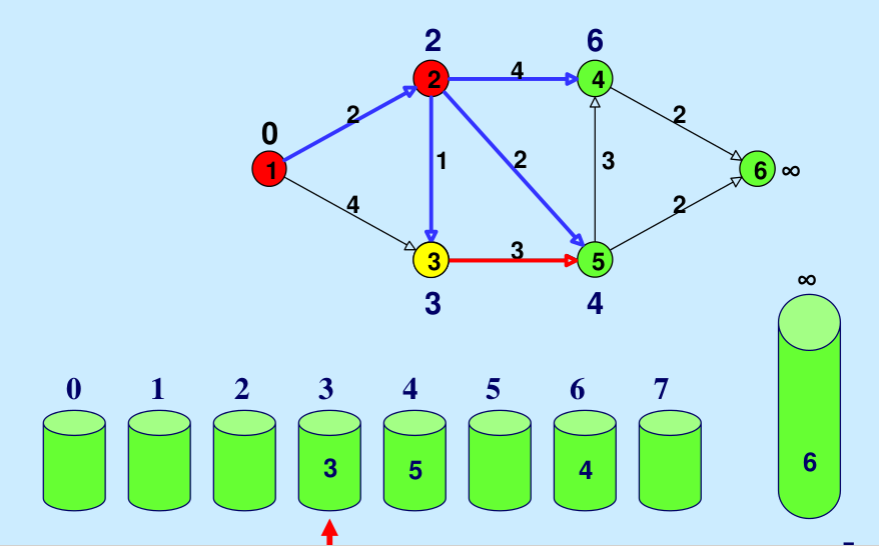
\includegraphics[width=\textwidth]{dijkstra_bounded.png}
\end{figure}

Μπορούμε να υλοποιήσουμε τα buckets ως hash tables με keys τις αντίστοιχες κορυφές. Έτσι, το pop από το bucket και το insert σε νέο bucket, δηλαδή οι διαδικασίες που αφορούν τα updates των γειτόνων, είναι διαδικασίες που έχουν κόστος $O(1)$. Από την άλλη, για να βρούμε το πιο αριστερό άδειο bucket μπορεί να χρειαστεί να ελέγξουμε ενδιάμεσα buckets. Η μετακίνηση όμως είναι μονότονη από αριστερά προς τα δεξιά που σημαίνει ότι κάθε φορά δεν χρειάζεται να ελέγξουμε buckets που είχαμε ελέγξει στο παρελθόν. Έτσι, η συνολική πολυπλοκότητα που θα δώσουμε για τη μετακίνηση στα buckets είναι $O(V \cdot C)$.
\bigbreak 

Στην χειρότερη περίπτωση θα πρέπει να ψάξουμε όλα τα buckets και να κάνουμε ένα decrease key operation για κάθε ακμή. Για να περάσουμε από όλα τα buckets θέλουμε πολυπλοκότητα $O(V\cdot C)$ ενώ αφού το decrease key θέλει $O(1)$ άμα τα buckets υλοποιηθούν με hash tables, το να κάνουμε decrease key για όλες τις ακμές θέλει πολυπλοκότητα $O(E)$. Έτσι, η συνολική πολυπλοκότητα είναι $O(E + V\cdot C)$ ή με τους συμβολισμούς τις εκφώνησης:
$$
O(m + nC)
$$

\subsection{(β)}
Για να επιτύχουμε τη ζητούμενη πολυπλοκότητα πρέπει να περάσουμε από διάφορα λογικά βήματα, τα οποία εξετάζουμε αναλυτικά στη συνέχεια.  \bigbreak 

Αρχικά, δηλώνουμε ότι ως ουρά προτεραιότητας θα χρησιμοποιήσουμε ένα σωρό. Ακόμη, δηλώνουμε ότι στην ουρά προτεραιότητας δεν θα έχουμε κορυφές αλλά buckets από κορυφές καθένα από τα οποία αντιστοιχεί σε μία απόσταση που έχει αποδοθεί στις κορυφές όσο τρέχει ο Dijkstra. \bigbreak 

Στη συνέχεια, θα αποδείξουμε ότι το πλήθος των κορυφών buckets που μπορούν να μπούν ταυτόχρονα μέσα στο heap δεν ξεπερνά το $2^C$ ή ισοδύναμα ότι δεν μπορούν να υπάρξουν συγχρόνως πάνω από $2^C$ διαφορετικές εκτιμήσεις για τις κορυφές όσο τρέχει ο Dijkstra.
\begin{lemma}Tο πλήθος των διαφορετικών εκτιμήσεων που μπορεί να δώσει ανά πάσα στιγμή ο Dijkstra στις κορυφές του γράφου φράσσεται από το $2^C$ αν όλα τα βάρη των κορυφών φράσσονται από το $2^C$. \end{lemma}

\begin{proof}
	\item 
	Κάθε στιγμή στον αλγόριθμο του Dijkstra, $\exists a \in \mathcal{N}$ για τον οποίο όλες οι ακμές που απέχουν πάνω από $a$ έχουν μπει στο κλειστό σύνολο. Οι κορυφές που περιέχονται στο priority Queue είναι αυτές που βρίσκονται σε απόσταση 1 ακμής από αυτές, καθώς αυτές είναι οι επόμενες που πρόκειται να γίνουν finalize. Άρα, οι αποστάσεις των κορυφών στο priority Queue είναι στο διάστημα $\{a+1, ..., a + 2^C\}$. Οι διαφορετικές αποστάσεις στο διάστημα αυτό φράσσονται από το $2^C$.
\end{proof}

Αφού δείξαμε ότι κάθε φορά υπάρχουν το πολύ $2^C$ διαφορετικές αποστάσεις στο priority queue, θα υπάρχουν και το πολύ $2^C$ διαφορετικά buckets που αντιστοιχούν σε αυτές τις αποστάσεις. Άρα, το priority queue θα έχει κάθε φορά το πολύ $2^C$ διαφορετικά στοιχεία. \bigbreak

Η αναζήτηση για το minimum σε σωρό έχει λογαριθμικό κόστος, άρα $O(log_22^C) = O(C)$. Επίσης, η πράξη του decrease key αντιστοιχεί στο να βρούμε το αντίστοιχο bucket να πάρουμε ένα στοιχείο του και αφού υπολογίσουμε την νέα τιμή του σε O(1) να βρούμε το νέο bucket και να το βάλουμε (αν το παλιό bucket άδειασε το πετάμε). Δηλαδή, αντιστοιχεί σε 2 αναζητήσεις και 1 delete στο σωρό που σημαίνει $O(C)$. \bigbreak

Η πολυπλοκότητα του Dijkstra όμως είναι:
$$
O(m\cdot T_{dk} + n\cdot T_{em}), \quad T_{dk}: \textrm{ χρόνος decrease key}, \quad T_{em}: \textrm{ χρόνος extract minimum}
$$

το οποίο όπως εξηγήσαμε γράφεται για την περίπτωση μας:
$$
O( (m+n) C)
$$
\section{Άσκηση 3}
\subsection{(α)}
\subsubsection{Διατύπωση αλγορίθμου}

Πριν διατυπώσουμε τον αλγόριθμο μας, είναι χρήσιμο να διατυπώσουμε μια αναδρομική σχέση για το πρόβλημα που θα μας βοηθήσει να καταστρώσουμε το σχέδιο αντιμετώπισης του. Έχουμε ότι:
$$
OPT(v, c) = min \big( OPT(u, c-c_{uv}) + w_{uv}, \quad \forall u: (u,v) \in E \big)
$$
Αυτή η σχέση αποτελεί μια γενίκευση της έννοιας του συντομότερου μονοπατιού που αποθηκεύει και το κόστος για την εύρεση του. Αν θέσουμε όλα τα κόστη $c_{ij}=0$ αυτό που παίρνουμε είναι η γνωστή μας σχέση με βάση την οποία κάνουμε τα updates στον Dijkstra. Αυτή λοιπόν η σχέση μας δίνει το πώς θα κάνουμε τα updates σε έναν γενικευμένο Dijkstra που δεν εκτελείται πάνω στις κορυφές του αρχικού γράφου αλλά πάνω σε states κορυφών. \bigbreak

Πιο συγκεκριμένα, θα θεωρήσουμε ότι ο Dijkstra διατηρεί δύο δομές, το ανοικτό μέτωπο και το κλειστό σύνολο. Το ανοικτό μέτωπο είναι ένα σύνολο με προτεραιότητες γενικευμένων κορυφών ως προς το μήκος, οι οποίες κορυφές δεν έχουν επεκταθεί πλήρως. Το κλειστό σύνολο είναι ένα σύνολο γενικευμένων κορυφών που έχουν επεκταθεί πλήρως. Με τον όρο γενικευμένες κορυφές εννοούμε κορυφές που κωδικοποιούν δύο πληροφορίες: το σε ποιά κορυφή του αρχικού γράφου αντιστοιχούν καθώς και το κόστος τους. \bigbreak 


Κάθε φορά διαλέγουμε από το ανοικτό μέτωπο το ποιά κορυφή θα χρησιμοποιηθεί με βάση τη διάταξη που ορίζουν οι προτεραιότητες. Στη συνέχεια για αυτή την γενικευμένη κορυφή πραγματοποιούμε τα updates όπως ορίζει η αναδρομική σχέση. Συγκεκριμένα, βρίσκουμε τις γειτονικές της κορυφές στον αρχικό γράφο. Αν οι γενικευμένες κορυφές που προκύπτουν από τους γείτονες της βάζοντας το κόστος της κορυφής που εξετάζουμε + το κόστος της σύνδεσης, δεν υπάρχουν στο Q, τότε τις προσθέτουμε με τις κατάλληλες προτεραιότητες. Αν πάλι υπάρχουν στο Q τότε κάνουμε τα απαραίτητα updates. \bigbreak 

Μόλις τελειώσει η εκτέλεση του Dijkstra κοιτάσουμε το κλειστό σύνολο και κρατάμε από αυτό μόνο τις γενικευμένες κορυφές που αντιστοιχούν στην κορυφή t. Διατάσσουμε ως προς τις προτεραιότητες τις κορυφές που απέμειναν. Εξετάζουμε μία μία αυτές τις γενικευμένες κορυφές από την μικρότερη προτεραιότητα (μικρότερο μήκος συντομότερου μονοπατιού) στη μεγαλύτερη. Η πρώτη από αυτές που θα βρούμε που δεν παραβιάζει το κριτήριο του κόστους είναι η λύση στο πρόβλημα μας.
\subsubsection{Απόδειξη ορθότητας}
Η ορθότητα του αλγορίθμου μας προκύπτει ως μια επέκταση της ορθότητας του αλγορίθμου του Dijkstra. Συγκεκριμένα, από τον τρόπο που κάνουμε τα updates γνωρίζουμε κάθε φορά ότι κάθε διαφορετικό κόστος που μπορεί να προκύψει από μονοπάτια κορυφών θα σχηματιστεί αφού οι κορυφές που αντιστοιχούν σε αυτό θα μπουν στο ανοικτό μέτωπο Q. Αφού κάθε φορά βάζουμε όλα τα προκύπτοντα κόστη που δεν υπάρχουν στο Q, ακόμα και αν αντιστοιχούν σε μεγαλύτερη προτεραιότητα, γνωρίζουμε ότι δεν θα χάσουμε κάποιο συνδυασμό κόστους και προτεραιότητας. \bigbreak 

Πέρα από την πληρότητα των συνδυασμών που εξασφαλίζει ο αλγόριθμος μας, το γεγονός ότι οι διάφορες κορυφές γίνονται updated με τον τρόπο που ορίζει ο Dijkstra, διασφαλίζει ότι οι προκύπτοντες συνδυασμοί είναι βέλτιστοι, ότι δηλαδή για συγκεκριμένο κόστος αυτό είναι το συντομότερο μονοπάτι που μπορεί να επιτευχθεί. \bigbreak 

Τέλος, ορθή είναι και η επιλογή του καλύτερου μονοπατιού από το κλειστό σύνολο, αφού ξεκινάμε από τα συντομότερα μονοπάτια με τα μεγάλα πιθανώς κόστη και όσο δεν τα καταφέρνουμε να ικανοποιήσουμε τους περιορισμούς καταφεύγουμε σε μεγαλύτερα μονοπάτια με μικρότερα κόστη.



\subsubsection{Ανάλυση πολυπλοκότητας}
Αφού η διάταξη είναι μονοδιάστατη ο χρόνος $T_{em}$ παραμένει ίδιας πολυπλοκότητας με τον απλό Dijkstra που γνωρίζουμε ως προς το μέγεθος του ανοικτού μετώπου Q. Αν χρησιμοποιηθεί Fibonacci heap η πράξη αυτή αντιστοιχεί σε $Ο(log|V|')$, όπου |V|' το πλήθος των κορυφών που θα μπούν στο ανοικτό σύνολο. \bigbreak

Ακόμη, και το decrease key γίνεται μόνο ως προς τη μία διάσταση, αυτή της προτεραιότητας, άρα διατηρεί την πολυπλοκότητα του με τον παραδοσιακό Dijkstra ως προς το μέγεθος του ανοικτού μετώπου Q. Σε Fibonacci heap η πράξη αυτή γίνεται σε O(1). \bigbreak 

Πρακτικά, η υλοποίηση μας αντιστοιχεί σε έναν Dijkstra με augmented ακμές και κορυφές. Η πολυπλοκότητα του Dijkstra όπως ξέρουμε είναι: 

$$
O(|E|'\cdot T_{dk} + |V|'\cdot T_{em}), \quad T_{dk}: \textrm{ χρόνος decrease key}, \quad T_{em}: \textrm{ χρόνος extract minimum}
$$
Με όσα παρατηρήσαμε γράφεται:
$$
O(|E|' + |V|' log|V|')
$$

Πρέπει λοιπόν να προσδιορίσουμε το πλήθος των ακμών και των κορυφών. \bigbreak 
Αφού κάθε ακμή έχει κόστος το πολύ $1$, δεν υπάρχει περίπτωση να ξεπεράσουμε το κόστος $|E|$ αφού κάθε μονοπάτι θα περιέχει το πολύ $|E|$ ακμές του αρχικού γράφου. Έτσι, οι κορυφές πολλαπλασιάζονται με έναν παράγοντα $|E|$, δηλαδή:

$$
|V|' =  |V| \cdot |E|
$$

Ακόμη, και οι ακμές πολλαπλασιάζονται με τον ίδιο παράγοντα καθώς στον augmented γράφο η γειτνίαση διατηρείται. Άρα:
$$
|E|' = |E| \cdot |E| = |E|^2
$$

Άρα, η συνολική πολυπλοκότητα είναι:
$$
O(|E|^2 + |V||E|log(|V||E|) )
$$

H πολυπλοκότητα των υπολοίπων πράξεων παραλείπεται ως πολύ μικρή συγκρινόμενη με την προαναφερθείσα.
\subsection{(β)}
Στο ερώτημα αυτό δεν αλλάζουμε τον αλγόριθμο μας, συνεπώς αφού για την ορθότητα δεν κάναμε καμία υπόθεση για την φύση των βαρών, η ορθότητα μένει ανεπηρέαστη.

\subsubsection{Ανάλυση πολυπλοκότητας}
Αυτό που πραγματικά αλλάζει είναι η πολυπλοκότητα του αλγορίθμου μας. Ο λόγος είναι ότι ο αριθμός των κορυφών δεν φράσσεται από κάποιο εξαρχής γνωστό αριθμό για το πρόβλημα αλλά εξαρτάται κάθε φορά από τη φύση των βαρών. Συγκεκριμένα, το μόνο φράγμα που γνωρίζουμε για το πλήθος των κορυφών (δηλαδή για τα διαφορετικά πιθανά κόστη που μπορούμε να συναντήσουμε) είναι: 
$$
C = W \cdot |E|
$$
όπου W το μεγαλύτερο κόστος στο πρόβλημα. \bigbreak 

Με την ανάλυση αυτή, ο αλγόριθμος μας έχει πολυπλοκότητα:
$$
O(|E|\cdot C + |V|\cdot C \log(|V|\cdot C))
$$

Ο αλγόριθμος αυτός είναι \textbf{ψεύδοπολυωνυμικός}, αφού το C μπορεί να γίνει απείρως μεγάλο.
\section{Άσκηση 4}
\subsection{Κατασκευή γράφου}
Η συγκεκριμένη άσκηση αφορά τη μοντελοποίηση του προβλήματος σε γράφο και την επίλυση του προβλήματος μέγιστης ροής σε αυτόν. \bigbreak 

Το πρόβλημα που περιγράφεται στην εκφώνηση είναι ένα πρόβλημα ροής πολλών πηγών (διαφορετικές εταιρείες) με περιορισμό όμως στη δυνατότητα παραγωγής ροής από κάθε πηγή (χρήματα $c_i$). Για τη μοντελοποίηση του προβλήματος αυτού εισάγεται ένας νέος κόμβος s που μπορεί να στέλνει σε κάθε μία πηγή ξεχωριστά ροή μικρότερη ή ίση από το capacity της κάθε πηγής (εταιρείας). \bigbreak 

Στο επόμενο στάδιο εισάγονται κόμβοι για κάθε άνθρωπο και οι εταιρείες συνδέονται με τους ανθρώπους που μπορούν να συνδεθούν, πληροφορία που δίνεται από τα σύνολα ενδιαφέροντος $S_i$. Αφού κάθε άνθρωπος πρέπει να αφαιρεί μια μονάδα από το $c_i$ της εταιρείας $i$, το capacity όλων αυτών των συνδέσεων είναι 1. \bigbreak 


Τέλος, όλοι οι άνθρωποι συνδέονται με έναν κόσμο προορισμού t με το capacity όλων των συνδέσεων να είναι στο 1, ώστε να ικανοποιηθεί η απαίτηση κάθε άνθρωπος να παίρνει το πολύ 1 διαφήμιση. \bigbreak 

Όσα περιγράφηκαν φαίνονται σχηματικά στον ακόλουθο γράφο:
\begin{center}
	\begin{tikzpicture}[scale=0.2]
	\tikzstyle{every node}+=[inner sep=0pt]
	\draw [black] (5,-30.2) circle (3);
	\draw (5,-30.2) node {$s$};
	\draw [black] (22.9,-12.8) circle (3);
	\draw (22.9,-12.8) node {$comp_1$};
	\draw [black] (22.9,-24.2) circle (3);
	\draw (22.9,-24.2) node {$comp_2$};
	\draw [black] (22.9,-35.5) circle (3);
	\draw (22.9,-35.5) node {$comp_3$};
	\draw [black] (22.9,-47.8) circle (3);
	\draw (22.9,-47.8) node {$comp_m$};
	\draw [black] (48.2,-12.8) circle (3);
	\draw (48.2,-12.8) node {$p_1$};
	\draw [black] (48.2,-25.4) circle (3);
	\draw (48.2,-25.4) node {$p_2$};
	\draw [black] (48.2,-36.2) circle (3);
	\draw (48.2,-36.2) node {$P_3$};
	\draw [black] (67.7,-30.2) circle (3);
	\draw (67.7,-30.2) node {$t$};
	\draw [black] (48.2,-48.9) circle (3);
	\draw (48.2,-48.9) node {$p_n$};
	\draw [black] (50.44,-14.8) -- (65.46,-28.2);
	\fill [black] (65.46,-28.2) -- (65.2,-27.3) -- (64.53,-28.04);
	\draw (58.96,-21.01) node [above] {$1$};
	\draw [black] (51.11,-26.12) -- (64.79,-29.48);
	\fill [black] (64.79,-29.48) -- (64.13,-28.81) -- (63.89,-29.78);
	\draw (57.24,-28.37) node [below] {$1$};
	\draw [black] (51.07,-35.32) -- (64.83,-31.08);
	\fill [black] (64.83,-31.08) -- (63.92,-30.84) -- (64.22,-31.8);
	\draw (58.8,-33.75) node [below] {$1$};
	\draw [black] (50.37,-46.82) -- (65.53,-32.28);
	\fill [black] (65.53,-32.28) -- (64.61,-32.47) -- (65.3,-33.19);
	\draw (58.97,-40.03) node [below] {$1$};
	\draw [black] (7.15,-28.11) -- (20.75,-14.89);
	\fill [black] (20.75,-14.89) -- (19.83,-15.09) -- (20.52,-15.81);
	\draw (15.21,-21.98) node [below] {$c_1$};
	\draw [black] (7.84,-29.25) -- (20.06,-25.15);
	\fill [black] (20.06,-25.15) -- (19.14,-24.93) -- (19.46,-25.88);
	\draw (15.06,-27.74) node [below] {$c_2$};
	\draw [black] (7.88,-31.05) -- (20.02,-34.65);
	\fill [black] (20.02,-34.65) -- (19.4,-33.94) -- (19.11,-34.9);
	\draw (12.92,-33.41) node [below] {$c_3$};
	\draw [black] (7.14,-32.3) -- (20.76,-45.7);
	\fill [black] (20.76,-45.7) -- (20.54,-44.78) -- (19.84,-45.49);
	\draw (11.71,-39.48) node [below] {$c_m$};
	\draw [black] (25.9,-12.8) -- (45.2,-12.8);
	\fill [black] (45.2,-12.8) -- (44.4,-12.3) -- (44.4,-13.3);
	\draw (35.55,-12.3) node [above] {$1$};
	\draw [black] (25.1,-14.84) -- (46,-34.16);
	\fill [black] (46,-34.16) -- (45.75,-33.25) -- (45.07,-33.99);
	\draw (34.53,-24.99) node [below] {$1$};
	\draw [black] (25.05,-26.3) -- (46.05,-46.8);
	\fill [black] (46.05,-46.8) -- (45.83,-45.89) -- (45.13,-46.6);
	\draw (34.53,-37.03) node [below] {$1$};
	\draw [black] (25.64,-22.97) -- (45.46,-14.03);
	\fill [black] (45.46,-14.03) -- (44.53,-13.91) -- (44.94,-14.82);
	\draw (36.53,-19.01) node [below] {$1$};
	\end{tikzpicture}
\end{center}
\subsection{Διατύπωση αλγορίθμου}
Αφου το πρόβλημα μοντελοποιηθεί σε γράφο με τον τρόπο που περιγράφηκε στην παραπάνω ενότητα, η επίλυση του ανάγεται στην επίλυση του προβλήματος της μέγιστης ροής. Συγκεκριμένα, χρησιμοποιείται κάποιος αλγόριθμος εύρεσης μέγιστης ροής σε γράφο, εδώ θα χρησιμοποιηθεί ο Edmonds-Karp και αν η ροή που βγαίνει από το s (ή ισοδύναμα η ροή που καταλήγει στο t) είναι n, σημαίνει ότι όλοι οι άνθρωποι είδαν από μια διαφήμιση. \bigbreak 

Αν κάτι τέτοιο είναι εφικτό, τότε ο αλγόριθμος εύκολα αποφασίζει ποιός άνθρωπος είδε διαφήμιση ποιάς εταιρείας, βλέποντας ποιές από τις ακμές που συνδέουν εταιρείες με ανθρώπους έχουν ροή 1.

\subsection{Διατύπωση ορθότητας}
Η ορθότητα του αλγορίθμου Edmonds-Karp εγγυάται ότι στο γράφημα θα βρεθεί η μέγιστη ροή. Κάθε εταιρεία μπορεί να δώσει μόνο μέχρι $c_i$ ροή λόγω των συνδέσεων με την πηγή, οπότε καλύπτεται η πρώτη προδιαγραφή. Αυτή η ροή μπορεί να διοχετευθεί μόνο σε ανθρώπους του συνόλου ενδιαφέροντος της καθώς έτσι κατασκευάστηκε ο γράφος, οπότε καλύπτεται και η 2η προδιαγραφή. Ένας άνθρωπος δεν μπορεί να δει παραπάνω από μία διαφημίσεις αφού το capacity των εισερχόμενων συνδέσεων στους ανθρώπους είναι 1, οπότε καλύπτεται και η 3η προδιαγραφή. Η απόφαση επίλυσης του αρχικού προβλήματος από την επίλυση του προβλήματος μέγιστης ροής σε γράφο παίρνεται από την συνολική ροή στο t, δηλαδή από το πόσοι άνθρωποι πήραν ροή (αφού κάθε άνθρωπος δίνει ως 1 μονάδα ροής στο t), συνεπώς το κριτήριο είναι σύμφωνο με όσα ζητήθηκαν στην εκφώνηση. \bigbreak 

Από τα παραπάνω προκύπτει η ορθότητα του αλγορίθμου.



\subsection{Χρονική πολυπλοκότητα}
Η χρονική πολυπλοκότητα είναι το max της πολυπλοκότητας κατασκευής του γράφου και της πολυπλοκότητας του αλγορίθμου Edmonds-Karp για την εύρεση της μέγιστης ροής σε αυτόν και του backtracking για την αντιστοίχηση ανθρώπων σε εταιρείες.
\subsubsection{Πολυπλοκότητα κατασκευής γράφου}
Ο γράφος αναπαρίσταται με λίστα γειτνίασης. Άρα, η πολυπλοκότητα κατασκευής του είναι η πολυπλοκότητα της προσθήκης ακμών. Έχουμε συνολικά m εταιρείες που κάθε μία συνδέεται δυνητικά με n ανθρώπους. Άρα, από εδώ προκύπτουν $n\cdot m$ ακμές. Ακόμη, υπάρχουν άλλες n ακμές για τη σύνδεση των ανθρώπων με τον προορισμό και άλλες m ακμές για τη σύνδεση της πηγής με τις εταιρείες. Άρα συνολικά, έχουμε
$\Theta(n\cdot m)$ ακμές, και αντίστοιχα ίδια πολυπλοκότητα για την κατασκευή του γράφου. \bigbreak 

\underline{Σημείωση:} Συνολικά για τον γράφο έχουμε:
$$
|V| = \Theta(n+m) 
$$
$$
|E| = \Theta(n \cdot m)
$$

\subsubsection{Πολυπλοκότητα Edmonds-Karp}
Ο αλγόριθμος Edmonds-Karp έχει πολυπλοκότητα:
$$
O(|V|\cdot |E|^2) = O(n^3m^3)
$$
\subsubsection{Πολυπλοκότητα Backtracking}
Για το backtracking, εξετάζονται απλώς οι ακμές οπότε έχουμε πολυπλοκότητα: $$O(|E|) = O(n\cdot m)$$


\subsubsection{Συνολική πολυπλοκότητα}
Από τα παραπάνω προκύπτει ότι η συνολική πολυπλοκότητα είναι:

$$
O(|V|\cdot |E|^2) = O(n^3m^3)
$$

\section{Άσκηση 5}
Έστω ότι ζητείται να αποδειχθεί ότι ένα πρόβλημα $A \in \mathbf{NPC}$. Αν είναι γνωστό ότι ένα πρόβλημα $B \in \mathbf{NPC}$ τότε η εργασία οργανώνεται ως εξής:
\begin{enumerate}
	\item Γίνεται η υπόθεση ότι το πρόβλημα Α μπορεί να λυθεί "εύκολα" (σε πολυωνυμικό χρόνο)
	\item Το πρόβλημα Β μετασχηματίζεται με κατάλληλο τρόπο σε ένα στιγμιότυπο εισόδου για το πρόβλημα Α που άμα λυθεί, δίνει την λύση για το Β
	\item Αφού το Α λύνεται γρήγορα (πολυωνυμικά), τότε και το Β λύνεται γρήγορα λόγω του 2.
	\item Κάτι τέτοιο δεν ισχύει, αφού $B \in \mathbf{NPC}$ άρα το Α είναι τουλάχιστον το ίδιο δύσκολο με το B.
	\item Αν δειχθεί ότι η λύση του Α επαληθεύεται σε πολυωνυμικό χρόνο τότε $A \in \mathbf{NPC}$.
\end{enumerate}

\subsection{3-Διαμέριση}
Έστω ότι είναι δυνατό να λύσουμε σε πολυωνυμικό χρόνο το πρόβλημα της 3 διαμέρισης. Θα δείξουμε ότι τότε θα είναι δυνατό να λύσουμε σε πολυωνυμικό χρόνο το πρόβλημα της 2-διαμέρισης, το οποίο γνωρίζουμε ότι είναι \textbf{NPC} για να οδηγηθούμε σε άτοπο. \bigbreak 

Έστω ότι μας δίνεται ένα σύνολο A και θέλουμε να δούμε αν υπάρχει 2-διαμέριση για το σύνολο αυτό. Βρίσκουμε το άθροισμα του συνόλου αυτού, έστω $s$. Έτσι, θέλουμε εμείς να διαμερίσουμε το σύνολο σε δύο υποσύνολα αθροίσματος $\frac{s}{2}$. \bigbreak 

Προσθέτουμε στο σύνολο Α έναν ακόμα αριθμό, φτιάχνοντας το σύνολο Α', τον αριθμό $\frac{s}{2}$. Έτσι, το σύνολο Α' θα έχει άθροισμα:
$$
s' = s + \frac{s}{2} = \frac{3s}{2}
$$ 

Δίνουμε το Α' για επίλυση στο πρόβλημα της 3-Διαμέρισης. Αναμένουμε να ελέγξει αν μπορεί να σπάσει σε τρία υποσύνολα αθροίσματος $\frac{s}{2}$ το καθένα. Αφού το κάθε υποσύνολο θα πρέπει να έχει άθροισμα $\frac{s}{2}$, το στοιχείο που προσθέσαμε θα πρέπει να μπει σε ένα υποσύνολο μόνο του. Η ένωση των άλλων δύο ξένων υποσυνόλων θα μας δίνει το Α και καθένα από αυτά θα έχει άθροισμα $\frac{s}{2}$. Άρα, βρήκαμε τρόπο να σπάσουμε σε πολυωνυμικό χρόνο το Α σε δύο ξένα υποσύνολα με άθροισμα $\frac{s}{2}$ το καθένα. Αφού το πρόβλημα αυτό είναι \textbf{NPC} οδηγούμαστε σε άτοπο. \bigbreak 

Άρα, το πρόβλημα της 3-Διαμέρισης είναι τουλάχιστον όσο δύσκολο όσο το πρόβλημα της 2-Διαμέρισης. Όμως μια 3-Διαμέριση ελέγχεται σε χρόνο $O(n)$, δηλαδή πολυωνυμικό, άρα το πρόβλημα είναι \textbf{NPC}.



\subsection{Άθροισμα υποσυνόλου κατά προσέγγιση}
\subsection{Κύκλος Hamilton κατά Προσέγγιση}
Έστω ότι είναι δυνατό να βρεθεί πολυωνυμικά αν υπάρχει κύκλος Hamilton κατά προσέγγιση. Έχουμε ένα γράφο, έστω $G(V,E)$, για τον οποίο στόχος είναι να βρούμε αν υπάρχει κύκλος Hamilton. Μετασχηματίζουμε τον γράφο $G(V,E)$ στον γράφο $G'(V', E')$ ώστε να διατηρηθούν όλες οι κορυφές και όλες οι ακμές του γράφου G και να προστεθεί για κάθε κορυφή του γράφου G μια κορυφή και μια ακμή που συνδέει την νέα κορυφή με την παλιά. \bigbreak

Με τον μετασχηματισμό αυτό, λύνουμε το πρόβλημα του κύκλου Hamilton κατά προσέγγιση για τον νέο γράφο που σχηματίστηκε. Αν το πρόβλημα λύνεται, γνωρίζουμε ότι από τη λύση αφαιρόντας τις extra ακμές και τις κορυφές που προστέθηκαν θα πάρουμε κύκλο Hamilton αφού "αναγκαστικά" στον κύκλο Hamilton κατά προσέγγιση για κάθε κορυφή του γράφου G η μια φορά θα σπαταληθεί για να περάσει ο κύκλος από τις extra κορυφές καθώς ο μόνος τρόπος να περάσει είναι μέσα από τις παλιές κορυφές που τους αντιστοιχούν. \bigbreak 


Αντίστοιχα, αν το πρόβλημα δεν λύνεται τότε γνωρίζουμε ότι δεν υπάρχει κύκλος Hamilton στον αρχικό γράφο καθώς η ελαστικότητα του προβλήματος του κύκλου Hamilton κατά προσέγγιση ώστε να περνάμε από κάθε κορυφή μέχρι και 2 φορές μας επιτρέπει να βρούμε κύκλο Hamilton αν υπάρχει. \bigbreak 

Δείξαμε ότι το πρόβλημα του κύκλου Hamilton κατά προσέγγιση είναι τουλάχιστον το ίδιο δύσκολο με το πρόβλημα του κύκλου Hamilton. Όμως μια λύση του επαληθέυεται σε πολυωνυμικό χρόνο, άρα ανήκει στην NP κλάση και αφού είναι το τουλάχιστον το ίδιο δύσκολο με ένα NP complete τότε θα είναι και αυτό NP Complete.


\subsection{Ικανοποιησιμότητα με περιορισμούς}
Αρχικά θα αποδείξουμε ότι αν μπορούμε να λύσουμε το πρόβλημα 4-SAT, τότε μπορούμε να λύσουμε και το πρόβλημα 3-SAT. \bigbreak 

Έστω ότι μας δίνεται ένα στιγμιότυπο εκφώνησης ενός 3-SAT προβλήματος της μορφής:
$$
(x_1\vee x_2 \vee x_3) \wedge (x_4 \vee x_5 \vee x_6) \wedge ... (x_k \vee x_{k+1} \vee x_{k+2})
$$
Σημειώνουμε ότι $x_i, x_j$ πιθανώς ταυτίζονται ή το ένα είναι άρνηση του άλλου. Σε κάθε όρο συμπληρώνουμε ένα $\vee \neg x_i$ όπου το $x_i$ να είναι ο πρώτος επιμέρους όρος κάθε ευρύτερου όρου που συμμετέχει στην τομή. Έστω $\neg x_p, x_{p+1}, ..., x_{p+k}$ οι επιμέρους όροι των οποίων προσθέσαμε την άρνηση. Προσθέτουμε ακόμη τους εξής όρους:
$$
(\neg x_p \vee x_{p+1} \vee x_{p+2} \vee x_{p+3}), \quad (\neg x_{p+1} \vee x_{p} \vee x_{p+2} \vee x_{p+3}), ...
$$
για κάθε τετράδα. 
Αν δεν υπάρχουν διαθέσιμοι όροι για να συμπληρωθεί τετράδα τους φτιάχνουμε ως εξής:
$$
x_1 \vee \neg x_1 \vee x_1 \vee x_1
$$


Δίνουμε το μετασχηματισμένο στιγμιότυπο για επίλυση προς το πρόβλημα 4-SAT με περιορισμούς. Ο μόνος τρόπος να λύνεται το δεύτερο και να μην λύνεται το πρώτο είναι κάθε όρος του δεύτερου να είναι αληθής. Με τον τρόπο που διαλέξαμε να σχηματίσουμε τους όρους του στιγμιοτύπου κάτι τέτοιο δεν συμβαίνει. Επίσης, αποτρέπουμε την περίπτωση να λυθεί το δεύτερο και να μη λύνεται το πρώτο καθώς οι περιορισμοί του προβλήματος θα αποτύγχουν σε μια τέτοια εκδοχή στους τελευταίους όρους που προσθέσαμε. \bigbreak 

Άρα, το 4-SAT με περιορισμούς πρόβλημα αν λύνεται μας δίνει λύση του 3-SAT που ξέρουμε ότι είναι \textbf{NPC}, δηλαδή το 4-SAT με περιορισμούς πρόβλημα είναι τουλάχιστον το ίδιο δύσκολο με το 3-SAT. Τα δύο προβλήματα είναι όμως ακριβώς ίδιας δυσκολίας αφού και για το $4-SAT$ με περιορισμούς μια λύση του επαληθεύεται σε πολυωνυμικό χρόνο και άρα ανήκει στην κλάση NP.
\subsection{Επιλογή ανεξάρτητων υποσυνόλων}
Θα δείξουμε ότι άμα μπορούμε να σπάσουμε σε k ξένα υποσύνολα τότε μπορούμε να λύσουμε και το 3DM πρόβλημα που γνωρίζουμε ότι είναι \textbf{NPC}. \bigbreak 
Έστω ένας τριμερής γράφος που αποτελείται από τα ξένα σύνολα $X, Y, Z$ για τον οποίο επιχειρούμε να βρούμε το μεγαλύτερο $3DM$. Παίρνουμε m ανεξάρτητα υποσύνολα πλειάδων από το σύνολο των πλειάδων του τριμερούς γραφήματος. Λύνουμε το πρόβλημα της επιλογής ανεξάρτητων υποσυνόλων για $k = |X| = |Y| = |Z|$ και έτσι παίρνουμε το τρισδιάστατο perfect matching. \bigbreak 

Δείξαμε ότι η επιλογή ανεξάρτητων υποσυνόλων είναι τουλάχιστον το ίδιο δύσκολη με το $3DM$. Όμως, μια λύση του προβλήματος αυτού επαληθεύεται σε πολυωνυμικό χρόνο άρα ανήκει στην κλάση NP και συνεπώς και τα δύο προβλήματα είναι \textbf{NPC}.

\nocite{*}
\bibliographystyle{plain}
\bibliography{ref}
\end{document}